\section{Аналитическая часть}

\noindent
\hspace{1.25cm}
В данном разделе проводится формализация задачи хранения истории деформаций трубчатых поверхностей и формализация данных, рассматриваются систем управления базами данных и обосновывается выбор решения для поставленной задачи.

\subsection{Постановка задачи}

\noindent
\hspace{1.25cm}
Дана трубчатая поверхность $T$, представляющая собой упорядоченное множество сечений $S = \{S_1, S_2, ..., S_m\}$, соединенных сегментами $\Gamma$. Каждое сечение $S_i$ определяется набором точек $P_i = \{p_{i1}, p_{i2}, ..., p_{in_i}\}$ в трехмерном пространстве, где $p_{ij} = (x_{ij}, y_{ij}, z_i)$. Сегмент $\Gamma_k$ между сечениями $S_k$ и $S_{k+1}$ содержит множество ребер $E_k = \{e_{k1}, e_{k2}, ..., e_{kl}\}$, соединяющих точки соседних сечений. Конечные точки ребра $e_{kj}$ не обязательно являются вершинами сечений, а могут лежать на ребрах сечений.

\noindent
\hspace{1.25cm}
Трубка характеризуется кривой центров $C = \{c_1, c_2, ..., c_m\}$, где центр $i$-го сечения определяется как:

\begin{equation}
c_i = \frac{1}{n_i} \sum_{j=1}^{n_i} p_{ij}
\end{equation}

\noindent
\hspace{1.25cm}
Требуется реализовать процесс деформации трубки с сохранением истории изменений геометрии. Далее рассмотрены этапы процесса деформации.

\noindent
\hspace{1.25cm}
\textbf{1. Выбор точки деформации}

\noindent
\hspace{1.25cm}
На кривой центров $C$ выбирается точка деформации $p_{def}$ с координатами $(x_{def}, y_{def}, z_{def})$.

\noindent
\hspace{1.25cm}
\textbf{2. Определение целевой точки}

\noindent
\hspace{1.25cm}
На плоскости $z = z_{def}$ выбирается целевая точка $p_{target}$ с координатами $(x_{target}, y_{target}, z_{def})$, определяющая направление и величину деформации. Вектор смещения вычисляется как:

\begin{equation}
\vec{d} = p_{target} - p_{def} = (x_{target} - x_{def}, y_{target} - y_{def}, 0)
\end{equation}

\noindent
\textbf{3. Применение локальной деформации с затуханием}

\noindent
\hspace{1.25cm}
К кривой центров применяется локальная деформация с функцией затухания. Для каждого центра $c_i$ вычисляется евклидово расстояние до точки деформации:

\begin{equation}
r_i = \sqrt{(x_i - x_{def})^2 + (y_i - y_{def})^2 + (z_i - z_{def})^2}
\end{equation}

\noindent
\hspace{1.25cm}
Вес влияния деформации определяется функцией затухания:

\begin{equation}
w_i(r) = e^{-\frac{r^2}{2\sigma^2}}
\end{equation}

где $\sigma$ -- радиус влияния деформации.

\noindent
\hspace{1.25cm}
Новое положение центра $i$-го сечения вычисляется по формуле:

\begin{equation}
c'_i = c_i + w_i(r_i) \cdot \alpha \cdot \vec{d}
\end{equation}

где $\alpha$ -- коэффициент силы деформации, $0 \leq \alpha \leq 1$.

\noindent
\hspace{1.25cm}
Деформированная кривая центров $C' = \{c'_1, c'_2, ..., c'_m\}$ образует новую осевую линию трубки.

\noindent
\textbf{4. Построение новых сечений}

\noindent
\hspace{1.25cm}
Для каждого деформированного центра $c'_i$ необходимо построить новое сечение, перпендикулярное касательной к кривой центров в данной точке.

\noindent
\hspace{1.25cm}
Вектор касательной к кривой в точке $i$ определяется методом центральных разностей:

\begin{equation}
\vec{\tau}_i = \begin{cases}
\frac{c'_{i+1} - c'_i}{||c'_{i+1} - c'_i||}, & i = 1 \\
\frac{c'_i - c'_{i-1}}{||c'_i - c'_{i-1}||}, & i = m \\
\frac{c'_{i+1} - c'_{i-1}}{||c'_{i+1} - c'_{i-1}||}, & 1 < i < m
\end{cases}
\end{equation}

\noindent
\hspace{1.25cm}
Плоскость нового сечения определяется уравнением:

\begin{equation}
\vec{\tau}_i \cdot (P - c'_i) = 0
\end{equation}

где $P = (x, y, z)$ -- произвольная точка плоскости.

\noindent
\hspace{1.25cm}
Точки исходного сечения $S_i$ проецируются на новую плоскость с сохранением их относительного положения относительно центра.

\subsection{Формализация данных}

\noindent
\hspace{1.25cm}
Исходя из сформулированных требований, база данных должна содержать информацию о таких объектах, как точка, сечение, ребро, сегмент и трубка.

\noindent
\hspace{1.25cm}
\textbf{1. Точка}

\noindent
\hspace{1.25cm}
Точка содержит сведения о координатах в трехмерном пространстве $(x, y, z)$ и порядковом номере внутри сечения.

\noindent
\hspace{1.25cm}
\textbf{2. Сечение}

\noindent
\hspace{1.25cm}
Сечение состоит из упорядоченного списка точек. Благодаря его упорядоченности, появляется возможность не хранить данные о ребрах сечения, так как ребра образуются посредством соединения точек с соседними индексами. Сечение содержит данные о координатах центра сечения $(x_{cen}, y_{cen}, z_{cen})$ и порядковом номере сечения в трубке.

\noindent
\hspace{1.25cm}
\textbf{3. Ребро}

\noindent
\hspace{1.25cm}
Ребро соединяет две точки соседних сечений и содержит сведения о длине ребра и порядковом номере в сегменте.

\noindent
\hspace{1.25cm}
\textbf{4. Сегмент}

\noindent
\hspace{1.25cm}
Сегмент состоит из упорядоченного списка ребер, соединяющих соседние сечения и содержит сведения о порядковом номере в трубке.

\noindent
\hspace{1.25cm}
\textbf{5. Трубка}

\noindent
\hspace{1.25cm}
Трубка объединяет сечения и сегменты и хранит общую длину трубки.

\noindent
\hspace{1.25cm}
При применении операции деформации к трубчатой поверхности изменяются координаты точек сечений, что приводит к необходимости сохранения новой версии геометрии. Для отслеживания истории таких изменений каждый геометрический объект также сохраняет номер версии и ссылки на предыдущую и следующую версии объекта.

\noindent
\hspace{1.25cm}
На рисунке~\ref{fig:er} представлена ER-диаграмма сущностей.

\begin{figure}[H]
\centering
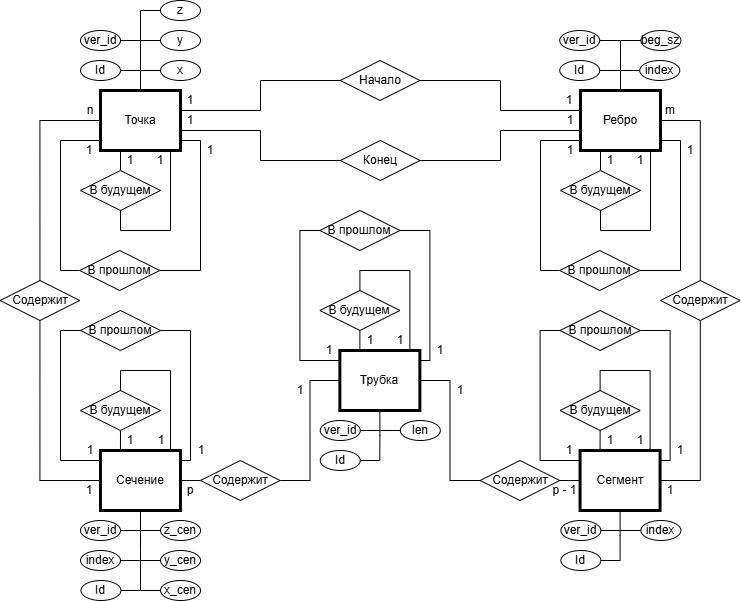
\includegraphics[width=1.0\textwidth]{img/er.png}
\caption{ER-диаграмма сущностей}
\label{fig:er}
\end{figure}

\subsection{Выбор модели данных}

\noindent
\hspace{0.75cm}
Модель данных~---~это совокупность абстракций и методов, с помощью которых мы стремимся имитировать понятия реального мира~\cite{komarov}.

\subsubsection{Реляционная модель}

\noindent
\hspace{1.25cm}
Реляционные СУБД (PostgreSQL, MySQL, Oracle) основаны на реляционной модели данных, где информация организуется в таблицы, состоящие из строк и столбцов. Каждая таблица имеет определенную структуру, а связи между таблицами устанавливаются с помощью внешних ключей~\cite{vas_hus}.

\noindent
\hspace{1.25cm}
Реляционные СУБД обеспечивают:

\renewcommand{\labelitemi}{---}
\begin{itemize}
    \item строгую типизацию данных с контролем на уровне схемы;
    \item поддержку принципов ACID (атомарность, согласованность, изолированность, долговечность);
    \item механизмы обеспечения ссылочной целостности через внешние ключи;
    \item возможность определения сложных ограничений целостности (CHECK, UNIQUE);
    \item транзакционную модель с поддержкой уровней изоляции~\cite{vas_hus}.
\end{itemize}

\noindent
\hspace{1.25cm}
По способу обработки запросов реляционные СУБД делятся на:
\begin{itemize}
    \item \textbf{OLTP} (строковые) --- подходят для систем с частыми изменениями данных;
    \item \textbf{OLAP} (колоночные) --- подходят для частых запросов с объединениями таблиц~\cite{vas_hus}.
\end{itemize}

\subsubsection{Документо-ориентированная модель}

\noindent
\hspace{1.25cm}
Документо-ориентированные СУБД (MongoDB, CouchDB) хранят данные в виде документов, обычно в формате JSON или BSON. Каждый документ содержит пары ключ-значение и может иметь вложенную структуру~\cite{luchinina}.

\noindent
\hspace{1.25cm}
Документо-ориентированная модель обеспечивает, что:

\begin{itemize}
    \item документы в одной коллекции могут иметь различную структуру, что позволяет хранить разнородные данные без необходимости изменения схемы базы данных;
    
    \item иерархические данные могут быть естественным образом представлены внутри одного документа, что упрощает извлечение связанной информации без операций объединения таблиц;
    
    \item высокую скорость чтения относительно других видов СУБД за счет минимизации количества обращений к базе данных;
    
    \item значения полей не имеют жесткой привязки к типам данных, что может привести к ошибкам на уровне приложения.
\end{itemize}

\subsubsection{База данных временных рядов}

\noindent
\hspace{1.25cm}
БД временных рядов (InfluxDB, TimescaleDB, Prometheus) специализированы для хранения последовательных событий или измерений с временными метками~\cite{komarov}.

\noindent
\hspace{1.25cm}
Баз данных временных рядов обеспечивают, что:

\begin{itemize}
    \item данные организованы по времени создания;
    
    \item устаревшие данные автоматически удаляются на основе правил времени жизни (TTL).
\end{itemize}

\subsubsection{Объектно-ориентированная модель}

\noindent
\hspace{1.25cm}
Объектная модель БД (db4o, ObjectDB, Versant) строится на принципах объектно-ориентированного программирования, где данные хранятся в виде объектов с методами~\cite{eldar}.

\noindent
\hspace{1.25cm}
Объектно-ориентированных СУБД обеспечивают:

\begin{itemize}
    \item \textbf{естественное отображение объектов ---} объекты приложения сохраняются непосредственно в базу данных без необходимости преобразования в другую структуру;
    
    \item \textbf{инкапсуляцию ---} данные и методы объединены в единую сущность, что обеспечивает согласованность бизнес-логики;
    
    \item \textbf{наследование и полиморфизм;}
    
    \item \textbf{навигацию по ссылкам ---} связи между объектами реализуются через прямые ссылки.    
\end{itemize}
    

\subsubsection{Графовые базы данных}

\noindent
\hspace{1.25cm}
Графовые СУБД (Neo4j, OrientDB, ArangoDB) специализируются на хранении связей между объектами. Данные представляются в виде узлов (вершин) и связей между ними (ребер), что обеспечивает естественное представление сетевых структур~\cite{otradnov}.

\noindent
\hspace{1.25cm}
Графовые базы данных обеспечивают:

\begin{itemize}
    \item переход между связанными узлами выполняется за константное время независимо от размера графа;
    
    \item узлы и ребра могут иметь произвольные свойства, а структура графа может динамически изменяться без модификации схемы;
    
    \item \textbf{Отсутствие JOIN операций.}
\end{itemize}

\subsection{Выбор системы управления базами данных}

\noindent
\hspace{1.25cm}
Для хранения истории деформаций трубчатых поверхностей база данных должна обладать следующими свойствами:

\begin{itemize}
    \item \textbf{строгая типизация данных} --- наличие встроенных механизмов контроля типов данных на уровне СУБД;
    \item \textbf{ссылочная целостность} --- поддержка внешних ключей и автоматический контроль связей между таблицами;
    \item \textbf{поддержка ACID} --- гарантии атомарности, согласованности, изолированности и долговечности транзакций;
    \item \textbf{ограничения целостности} --- возможность определения ограничений на уровне схемы;
    \item \textbf{каскадные операции} --- автоматическое распространение операций удаления и обновления на связанные записи.
\end{itemize}

\begin{table}[H]
    \captionsetup{justification=raggedright, singlelinecheck=false}
    \caption{Сравнение моделей данных}
    \label{tbl:db_comparison}
    \begin{center}
        \begin{tabular}{|l|c|c|c|c|c|}
            \hline
            \textbf{Критерий} & \textbf{Реляц.} & \textbf{Докум.} & \textbf{Врем. р.} & \textbf{Объект.} & \textbf{Граф.} \\\hline
            Строгая типизация & + & $-$ & + & + & $-$ \\\hline
            Ссылочная целостность & + & $-$ & $-$ & + & $-$ \\\hline
            Поддержка ACID & + & $-$ & $-$ & + & $-$ \\\hline
            Ограничения целостности & + & $-$ & $-$ & + & $-$ \\\hline
            Каскадные операции & + & $-$ & $-$ & $-$ & $-$ \\\hline
        \end{tabular}
    \end{center}
\end{table}

\noindent
\hspace{1.25cm}
На основании проведенного сравнения для решения поставленной задачи необходимо выбрать реляционную модель СУБД.


\subsection{Вывод}

\noindent
\hspace{1.25cm}
В данном разделе была проведена формализация задачи хранения истории деформаций трубчатых поверхностей и формализация данных, были рассмотрены системы управления базами данных и был обоснован выбор решения для поставленной задачи.

\newpage